%\epigraph{Yesterday's rose stands only in name, we hold only empty names.}{--- \textup{Umberto Eco}, \textit{The Name of Rose}}
 

 Neutrinos are one of the elementary particles we currently know and are included in the Standard Model (SM). However, some properties of neutrinos can not be described by the SM, which shows clues of the new physics beyond the Standard Model.

SNO+ experiment is planned to explore one of the unknown properties of neutrinos: whether the neutrinos are Majorana particles or Dirac particles.



Massive neutrinos are discussed ...
\section{Neutrino Oscillation}

Neutrino oscillation was first discovered in 1998.
It is the first direct evidence showing that the Standard Model is incomplete. 


solar neutrino oscillations




matter effect





\section{Majorana Neutrino}

Dirac equation $(i\gamma^\mu\partial_\mu-m)\psi=0$,
get coupled equations


The interpretation of the $0\nu\beta\beta$ process is considered as exchanging light Majorana neutrinos. In this case the effective Majorana mass $<m_{ee}>=\sum_{i=1}^{3} |U_{ei}|^2m_i~(i=1,2,3)$, $U_{ei}$ are the elements of the neutrino mixing matrix for the flavor state $\nu_e$, and $m_i$ are the mass eigenvalues of the mass eigenstates (from (\ref{eq:mixingmatrix})). The observable quantity is the half-life:
\[
(T^{0\nu\beta\beta}_{1/2})^{-1} = G_{PS}(Q,Z)|M_{Nuclear}|^2<m_{ee}>^2, 
\]

Majorana found a representation of the $\gamma$-matrices as follow:
\[
\gamma_M^0 = \begin{pmatrix} 
0 & \sigma^2 \\
\sigma^2 & 0
\end{pmatrix},
\gamma_M^1 = \begin{pmatrix} 
\sigma^3 & 0 \\
0 & \sigma^3
\end{pmatrix},
\gamma_M^2 = \begin{pmatrix} 
-\sigma^2 & 0 \\
0 & \sigma^2
\end{pmatrix},
\gamma_M^3 = -i\begin{pmatrix} 
\sigma^1 & 0 \\
0 & \sigma^1
\end{pmatrix}
\]


These matrices themselves are pure imaginary. 




\section{Double Beta Decay}

For heavy radioactive isotopes with nuclei of even neutron number (N) and even proton number (Z) (called even-even nucleus), beta decay will lead to an odd-odd nucleus which is less stable. For some such isotopes the beta decay is energetically forbidden. In 1935, Maria Goeppert-Mayer pointed out that they can still decay through a double beta decay process: $(Z,A) \to (Z+2,A)+2e^{-}+2\bar{\nu_e}+Q_{\beta\beta}$, where the $Q_{\beta\beta}$ is the released energy. This is called ordinary double beta decay or $2\nu\beta\beta$, which is allowed by the Standard Model and with a typical half-life $T_{1/2}>10^{19}$ years\cite{martin}.

In 1937, Ettore Majorana proposed that neutral spin-1/2 particles (fermions) can be their own antiparticles\cite{majorana}. If neutrinos have this behaviour, the process called neutrinoless double beta decay ($0\nu\beta\beta$) will also be expected. The Feynman diagrams of $2\nu\beta\beta$ and $0\nu\beta\beta$ are illustrated in Figure~\ref{feynman1}.

%\begin{figure}[htbp]
%	\centering	
%	\begin{minipage}[t]{0.45\textwidth}
%		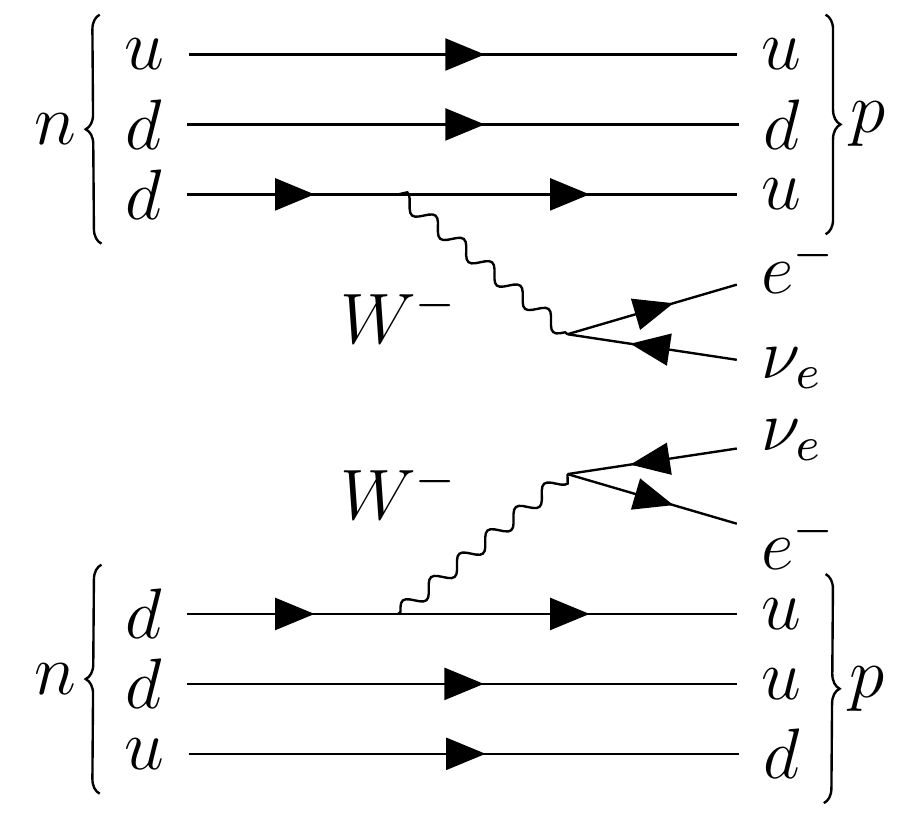
\includegraphics[width=5cm]{doubleBeta2nu_feynman.png}
%	\end{minipage}
%	\begin{minipage}[t]{0.45\textwidth}
%		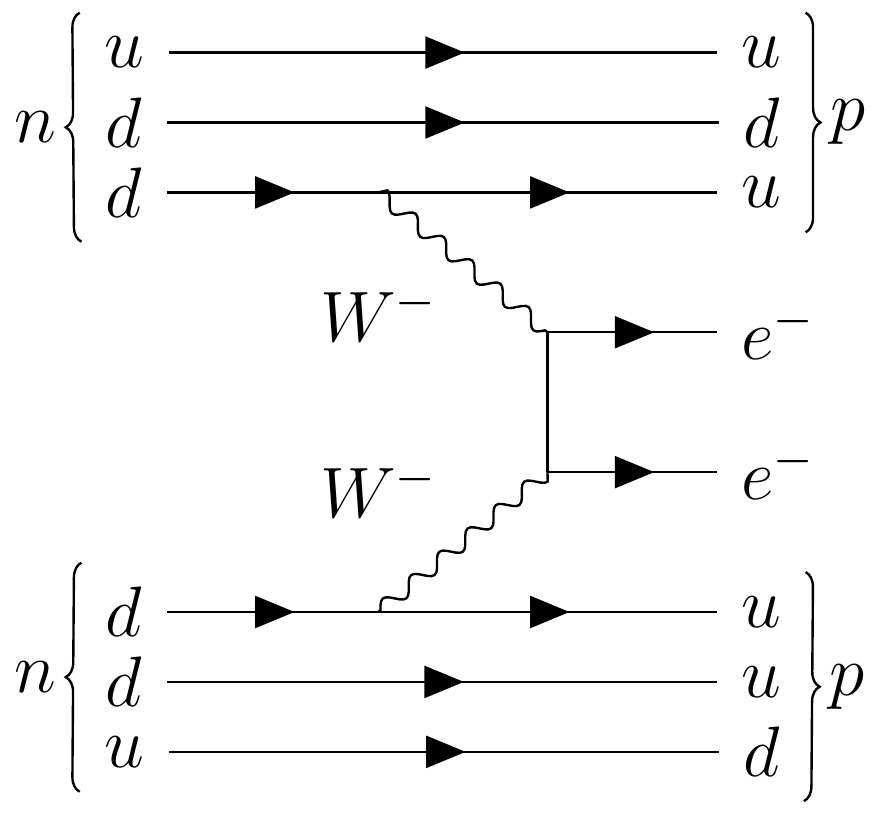
\includegraphics[width=5cm]{doubleBeta_feynman.png}
%	\end{minipage}
%	\caption{ Feynman diagrams for $2\nu\beta\beta$ (left) and $0\nu\beta\beta$ (right).}
%	\label{feynman1}
%\end{figure}

The interpretation of the $0\nu\beta\beta$ process is considered as exchanging light Majorana neutrinos. In this case the effective Majorana mass $<m_{ee}>=\sum_{i=1}^{3} |U_{ei}|^2m_i~(i=1,2,3)$, $U_{ei}$ are the elements of the neutrino mixing matrix for the flavor state $\nu_e$, and $m_i$ are the mass eigenvalues of the mass eigenstates (from (\ref{eq:mixingmatrix})). The observable quantity is the half-life:
\[
(T^{0\nu\beta\beta}_{1/2})^{-1} = G_{PS}(Q,Z)|M_{Nuclear}|^2<m_{ee}>^2, 
\]
where $G_{PS}$ is the phase space factor and $|M_{Nuclear}|$ is the nuclear matrix element for the physics process describing the $0\nu\beta\beta$ decay process\cite{kaizuber}.

Similar to beta decay, the $2\nu\beta\beta$ process will cause a continuous spectrum in the detector while the $0\nu\beta\beta$ process only has two electrons in the final state, which sum up to give a distinct energy peak. By measuring this exact energy, a detector with high energy resolution is able to search for the $0\nu\beta\beta$ signal from the $0\nu\beta\beta$ decay radioactive isotopes. Diverse technologies have been developed during the past decades. The following section lists some of the mainstream experiments.

\subsection{Status of Double Beta Decay Experiments}

At the time of writing, 

$0\nu\beta\beta$ in the range of $10^{25}-10^{26}$ year,











The GERmanium Detector Array (GERDA) experiment searches for $0\nu\beta\beta$ of $^{76}$Ge. The experiment uses bare germanium crystals with an enrichment of up to $\sim$87\% $^{76}$Ge operated in a radiopure cryogenic liquid argon (LAr). GERDA Phase I had an exposure of 21.6 kg$\cdot$yr and Phase-II started with 35.6kg from enriched material in December 2015. With combined data of Phase I and Phase II, 

a total exposure of 82.4 kg$\cdot$yr 



GERDA reported in 2019 a lower limit half-life of $T^{0\nu}_{1/2}(^{76}$Ge$)>0.9\times 10^{26}$ years at 90\% C.L.\cite{gerda,gerda2}.




The Enriched Xenon Observatory (EXO) experiment uses 200-kg liquid Xenon (LXe) time projection chamber (TPC) to search for $0\nu\beta\beta$ in $^{136}$Xe. In 2011 they observed the half life of double beta decay of $^{136}$Xe to be $2.11\times 10^{21}$ years and in 2014 they set a limit on $T^{0\nu}_{1/2}(^{136}$Xe$)>1.1\times 10^{25}$ yr\cite{exo}. EXO is now upgrading to the next 5-tonne experiment (nEXO) and is expected to reach an exclusion sensitivity of $T^{0\nu}_{1/2}(^{136}$Xe) to about $10^{28}$ years at 90\% C.L.\cite{nEXO}.

Also looking into $^{136}$Xe, the KamLAND-Zen (ZEroNeutrino) experiment exploits the existing facilities of KamLAND by setting a 3.08-m-diameter spherical inner balloon filled with 13 tons of Xe-loaded liquid scintillator at the center of the KamLAND detector.

liquid scintillator cocktail of 82\% decane and 18\% pseudocumene by volume, 2.7 g/L PPO.

photocathode coverage of 34\%.

 Their 2016 results from a 504 kg$\cdot$yr exposure obtained a lower limit for the $0\nu\beta\beta$ decay half-life of $T^{0\nu}_{1/2}(^{136}$Xe$)>1.07\times 10^{26}$ yr at 90\% C.L. and the corresponding upper limits on the effective Majorana neutrino mass are in the range 61-165 meV\cite{kamlandZen}.

The Particle and Astrophysical Xenon Experiment III (PandaX-III) 
high pressure gas-phase time projection chamber (TPC)  




The Cryogenic Underground Observatory for Rare Events (CUORE) experiment searches for $0\nu\beta\beta$ in $^{130}$Te. CUORE is a ton-scale cryogenic bolometer array that arranges 988 tellurium dioxide (TeO$_2$) crystals. CUORE reported first results in 2017 after a total TeO$_2$ exposure of 86.3 kg$\cdot$yr. Combined with their early data, they placed a lower limit of $T^{0\nu}_{1/2}(^{130}$Te$)>1.5\times 10^{25}$ yr at 90\% C.L. and $m_{\beta\beta}<(140-400)$  meV\cite{cuore}.

